%!TEX root = ../paper.tex

\begin{figure}
	\centering
	\begin{subfigure}{0.23\textwidth}
		\centering
		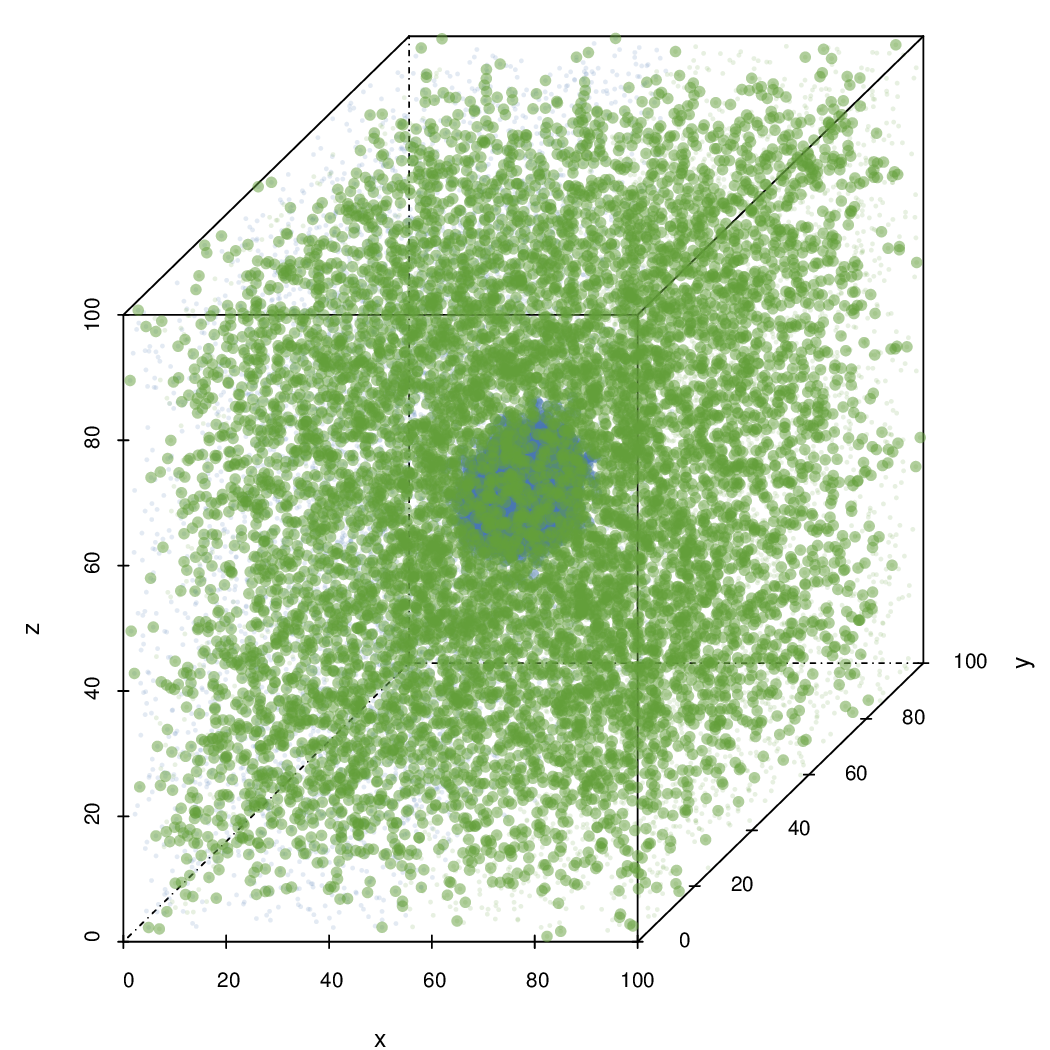
\includegraphics[keepaspectratio=true, width=\textwidth, height=0.23\textheight]{discussion/img/ferdosi_1_abs_error_mbeSmallerThansambe.pdf}
		\caption{Dataset \ferdosiOne}
		\label{fig:discussion:singleSphere:mbeLowerError:ferdosi1}
	\end{subfigure}
	\begin{subfigure}{0.23\textwidth}
		\centering
		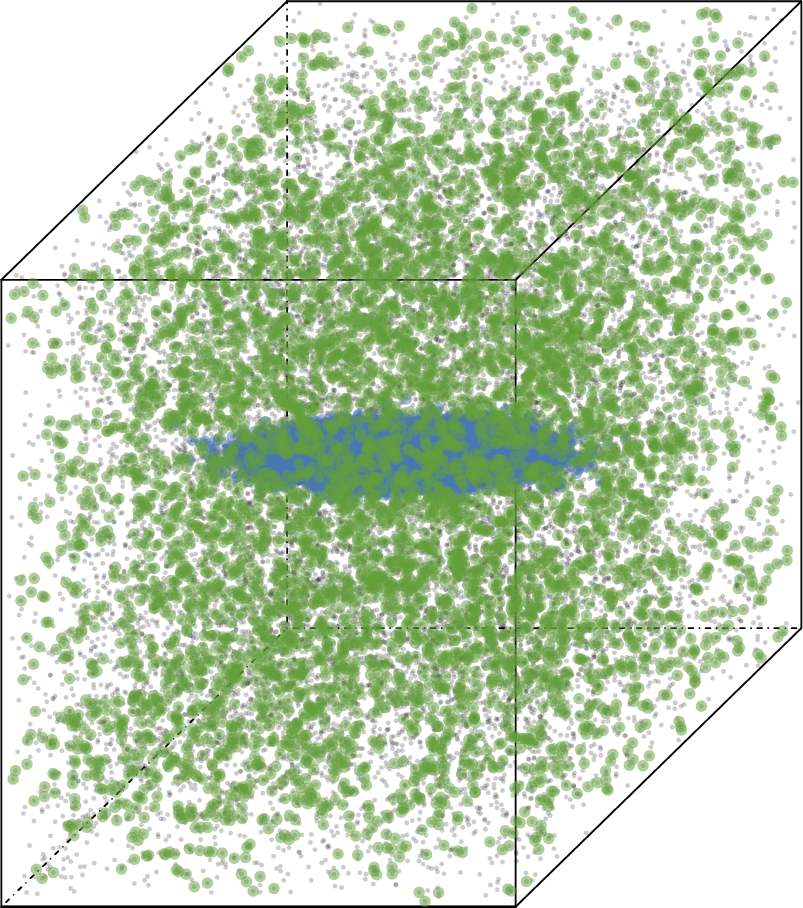
\includegraphics[keepaspectratio=true, width=\textwidth, height=0.23\textheight]{discussion/img/baakman_1_abs_error_mbeSmallerThansambe.pdf}
		\caption{Dataset \baakmanOne}
		\label{fig:discussion:singleSphere:mbeLowerError:baakman1}
	\end{subfigure}	
	\begin{subfigure}{0.23\textwidth}
		\centering
		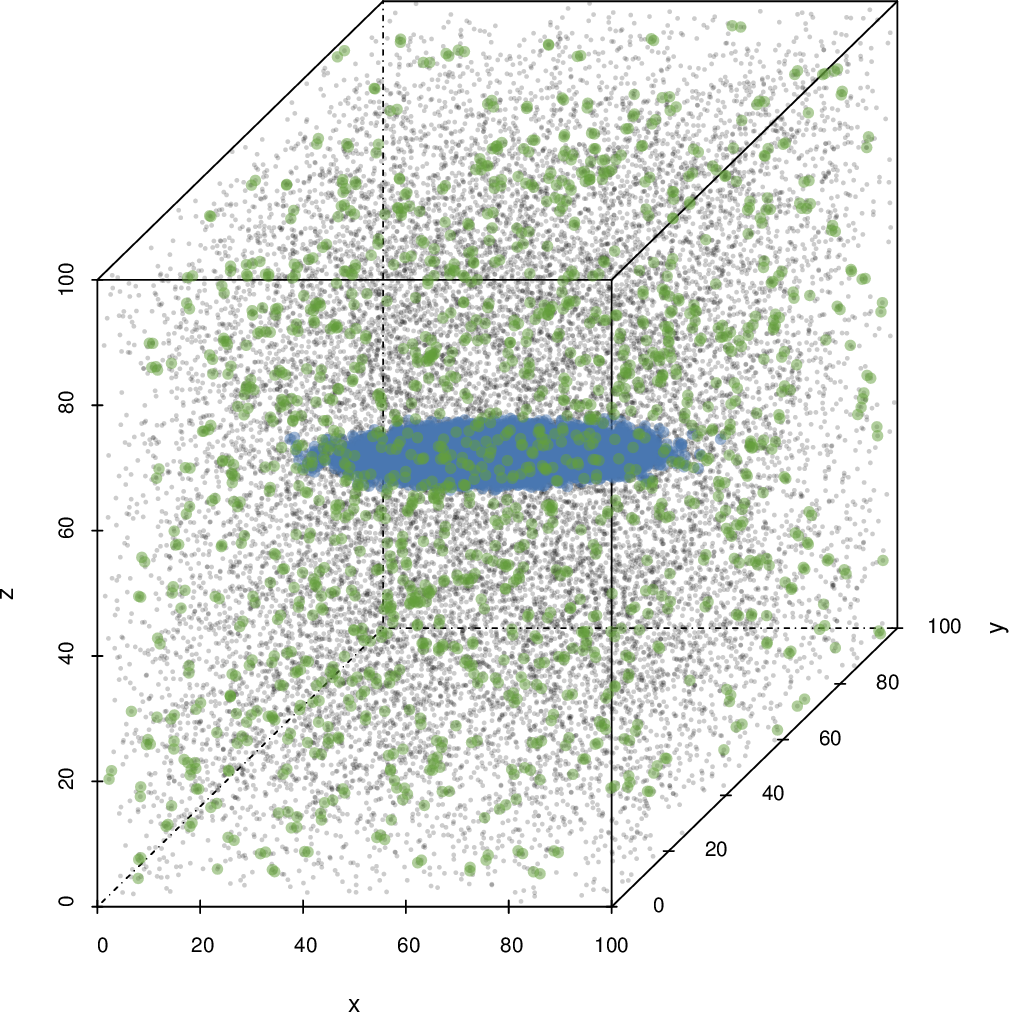
\includegraphics[keepaspectratio=true, width=\textwidth, height=0.23\textheight]{discussion/img/baakman_4_abs_error_mbeSmallerThansambe.pdf}
		\caption{Dataset \baakmanFour}
		\label{fig:discussion:singleSphere:mbeLowerError:baakman4}
	\end{subfigure}		
	\begin{subfigure}{0.23\textwidth}
		\centering
		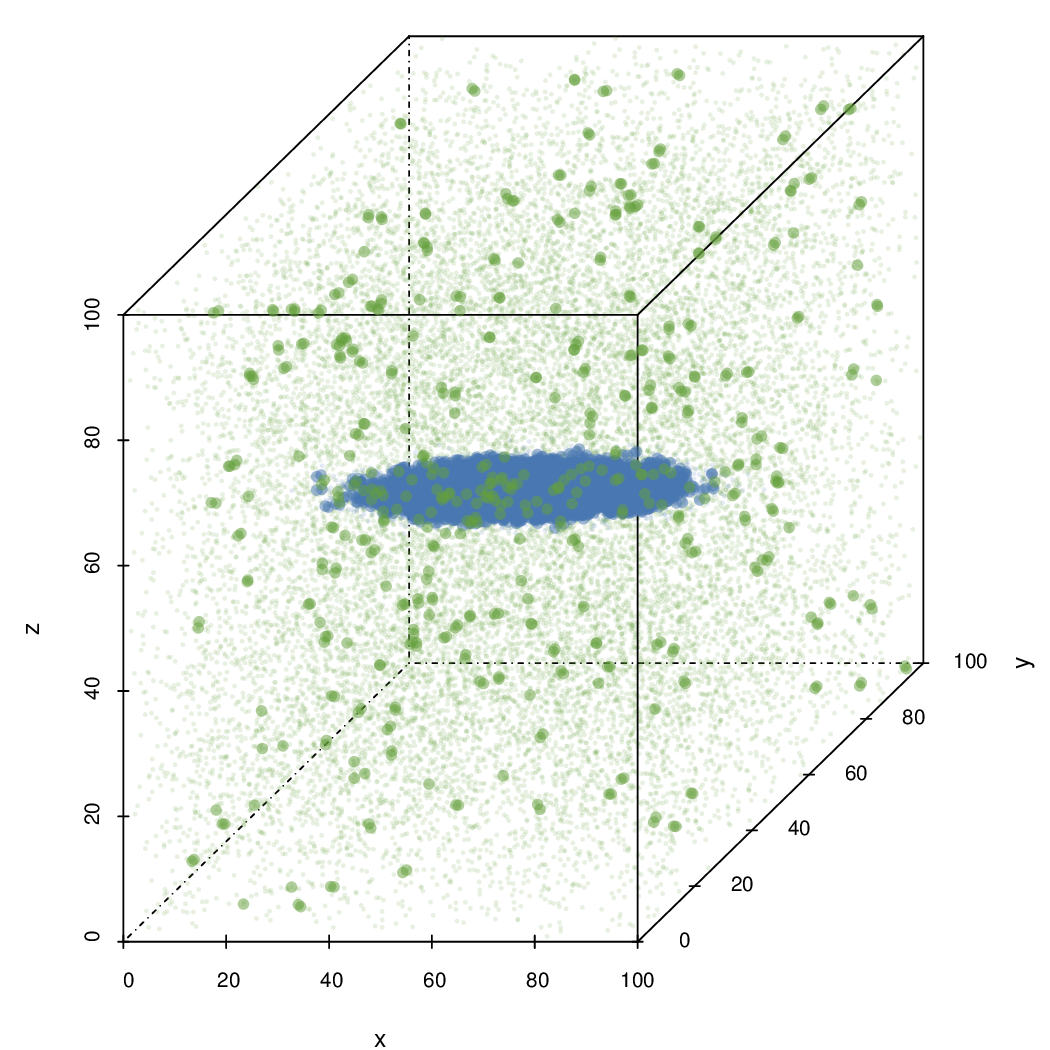
\includegraphics[keepaspectratio=true, width=\textwidth, height=0.23\textheight]{discussion/img/baakman_5_abs_error_mbeSmallerThansambe.pdf}
		\caption{Dataset \baakmanFive}
		\label{fig:discussion:singleSphere:mbeLowerError:baakman5}
	\end{subfigure}			
	\caption{Low opacity scatter plot of dataset %
		\subref{fig:discussion:singleSphere:mbeLowerError:ferdosi1} \ferdosiOne, %
		\subref{fig:discussion:singleSphere:mbeLowerError:baakman1} \baakmanOne, %
		\subref{fig:discussion:singleSphere:mbeLowerError:baakman4} \baakmanFour, and%
		\subref{fig:discussion:singleSphere:mbeLowerError:baakman5} \baakmanFive, %
		with an overlay of larger points with a higher opacity where the absolute error of \sambe is larger than the absolute error of \mbe.}
	\label{fig:discussion:singleSphere:mbeLowerError}
\end{figure}

% Introduction
The scatter plots of the datasets with a single Gaussian in \cref{fig:discussion:singleSphere:mbeLowerError} emphasize the points where the absolute error of the symmetric estimator is smaller than that of the shape-adaptive estimator. 

	% Ferdosi 1
		% The overlay plot
		\Cref{fig:discussion:singleSphere:mbeLowerError:ferdosi1} shows that the shape-adaptive estimator results outperforms the symmetric estimators on most points near the boundary of the dataset. It also seems to to illustrate that that \mbe results in a lower error than \sambe on the other points, however the raw data shows that on \num{52.72411}\% of the full dataset, and on \num{55.6575} \% of the Gaussian component the symmetric estimator results in a lower absolute error.
		% The shape of the kernels
		Reviewing the shape of the kernels used for the points in dataset \ferdosiOne we find that the used kernels are all near spherical. The kernels with the largest differences between their eigenvalues are associated with points near the boundary of the dataset. 
		% Largest differnces in estimated values between kernels. 
		The largest differences in error between the two estimators can be found near the center of the Gaussian component, where the shape-adaptive kernels are relatively spherical. The difference between the two estimators at these points is caused by the number of points used to estimate the density, for most of these points \sambe uses too many points which results in an overestimated density. 

	% Baakman 1
		% Overlay plot
		The results in \cref{fig:discussion:singleSphere:mbeLowerError:baakman1} are comparable to those in \cref{fig:experiment:singlesphere:ferdosi1}, however there seem to be fewer points of the noise component where the absolute error of using the symmetric-kernel is lower than using a shape-adaptive kernel. This is disproven by the raw data which shows that \num{51.41694}\% of the points of the noise component \mbe outperforms \sambe. 
		% The shape of the kernels
		As in dataset \ferdosiOne the points with the most ellipsoidal kernels are positioned near the boundaries of the dataset, where \sambe outperforms \mbe. 
		% Largest differences in estiamted values between kernels
		The points whose differences in estimated densities are largest are, as in dataset \ferdosiOne, found near the mean of the Gaussian distribution. These differences are mostly caused by the shape-adaptive estimator overestimating the densities of these points.

	%Baakman 4
	\todo[inline]{Wat zien we in het plotje?}
	\todo[inline]{Iets over de vorm van de kernels.}
	\todo[inline]{What is the influence of the distance to the mean?}

	%Baakman 5
	\todo[inline]{Wat zien we in het plotje?}
	\todo[inline]{Iets over de vorm van de kernels.}
	\todo[inline]{What is the influence of the distance to the mean?}

% General observations 
\todo[inline]{Waarom sambe zoveel beter op randen, zo veel slechter in de buurt van de mean van de distributie?}
	% Ferdosi 1

	% Baakman 1

	% Baakman 4

	% Baakman 5



\oldStuff

%General Discussion
	%Small difference between two estimators
		% Confirm with plots
		The most striking observation of \cref{s:results:singleGaussian} is the small difference between the densities approximated by the two estimators. To investigate what caused these differences, we first verified if the differences in \mse were caused by a select group of points, to that end we compared the density estimations of the individual points by plotting the results of \sambe as a function of \mbe. These plots do not indicate a specific group of points that causes the difference in \MSE between the two estimators within datasets.
		
		% Investigate the points with the largest differences
		Investigating the points that result in the biggest difference in estimated density between estimators we find that in the datasets with a single Gaussian they all lie near the mean of the Gaussian distribution. Furthermore the density of these points are both over and underestimated by the shape-adaptive estimator, if the first is the case generally fewer points have contributed to the \mbe density than to the \sambe density. If the shape-adaptive estimator underestimates densities it generally uses far less points to base its approximation on than the symmetric estimator uses for that same point. This suggest that some of the kernels near the mean of the Gaussian our to big, allowing a contribution to some points that they should not contribute to, and conversely that some are too small. 

		% Investigate the kernels.
		Reviewing the shape of the kernels used by the shape-adaptive estimator we find some differences between the datasets. 
			% Ferdosi 1
			In dataset \ferdosiOne, as expected due to the spherical Gaussian, the three eigenvalues of the kernels hardly differ, indicating that the kernels are near spherical. 
			% Baakman 1
			In the elongated version of this dataset, a couple of points have ellipsoidal kernels, as indicated by the eigenvalues of their covariance matrices. Since all these points are positioned in corners of the dataset we contribute the shape of these kernels to their position, instead of to any influence from the Gaussian distribution. This problem could possibly be solved by taking a larger neighborhood into account when determining the kernel shape. 
			% Baakman 4
			In dataset \baakmanFour numerous points have strongly ellipsoidal kernels, a lot of these points can be found at the boundaries of the datasets. However a lot of these point are also placed in and around the Gaussian distribution. 
			% Baakman 5
			The same holds for dataset \baakmanFive.
		%Some general blaat
		\todo[inline]{This is wrong! SAMBE works better at the boundaries for multisphere sets, quite likely also the case for single sphere.}	
		There is no way for the kernel determination algorithm to distinguish between points that lie at the edge of a dataset, or a point that lies at the boundary of the distribution. If the density of interest lies in large area of irrelevant points one could discard the estimated densities at the boundaries, since these suffer from this boundary-effect.
			
